\documentclass[UTF8,fontset=fandol,a4paper,zihao=-4]{ctexart}
\usepackage[a4paper,margin=2.5cm]{geometry}
\usepackage{amsmath,amssymb,amsthm,bm,booktabs,array,longtable,graphicx,float,enumitem,hyperref,fancyhdr,needspace,listings}
\usepackage{tikz}
\usetikzlibrary{arrows.meta,positioning,calc,shapes.geometric}
\lstset{basicstyle=\ttfamily\fontsize{7.5}{9}\selectfont,breaklines=true,breakatwhitespace=false,columns=fullflexible,keepspaces=true,showstringspaces=false,frame=single,numbers=left,numberstyle=\tiny,numbersep=5pt,tabsize=4,keywordstyle=\color{blue!55!black},commentstyle=\color{black!65},stringstyle=\color{green!35!black},captionpos=t,xleftmargin=1.5em}
\hypersetup{hidelinks,pdftitle={基于交会定位与覆盖搜索的无线电干扰源清除策略},pdfauthor={}}
\graphicspath{{b_solution/report/figures/}}
\setlength{\parindent}{2em}
\setlength{\parskip}{0.1em}
\setlength{\emergencystretch}{2em}
\linespread{1.18}
\setlist{itemsep=0.25em,topsep=0.35em,parsep=0pt}
\setlength{\textfloatsep}{12pt plus 2pt minus 2pt}
\setlength{\floatsep}{10pt plus 2pt minus 2pt}
\pagestyle{fancy}\fancyhf{}\fancyfoot[C]{\thepage}
\renewcommand{\headrulewidth}{0pt}
\DeclareMathOperator{\conv}{conv}
\DeclareMathOperator*{\argmin}{arg\,min}
\newcommand{\norm}[1]{\left\lVert#1\right\rVert}
\newcommand{\cross}[2]{\operatorname{cross}(#1,#2)}
\newcommand{\disk}{\mathcal D}
\newcommand{\poly}{\mathcal P}
% 由已保存的逐世界结果计算，单位和分母见各表标题。
\newcommand{\QThreeControlMean}{258.99}
\newcommand{\QThreeControlPooled}{254.41}
\newcommand{\QThreeFieldMean}{250.17}
\newcommand{\QThreeFieldPooled}{245.65}
\newcommand{\QThreeSaving}{8.82}
\newcommand{\QThreeGain}{3.40}
\newcommand{\QThreeLow}{8.01}
\newcommand{\QThreeHigh}{9.62}
\newcommand{\QThreeWins}{827}
\newcommand{\FormalThree}{
\begin{tabular}{clrrrr}
\toprule
次数 & 案例编码 & $K$ & $T$/秒 & $T/K$/秒 & 本机运行/秒 \\
\midrule
1 & \texttt{UAKK-9823-A2SU-2CNM} & 14 & 3136.520 & 224.037 & 0.7665 \\
2 & \texttt{5CV9-WP56-W8T6-YMBM} & 10 & 2701.627 & 270.163 & 0.8526 \\
3 & \texttt{PNKS-Z5H4-TW3T-FDV6} & 16 & 3450.360 & 215.647 & 0.8749 \\
\bottomrule
\end{tabular}
}
\newcommand{\FormalThreeK}{40}
\newcommand{\FormalThreeT}{9288.507}
\newcommand{\FormalThreeMean}{236.616}
\newcommand{\FormalThreePooled}{232.213}
\newcommand{\QFourControlMean}{542.41}
\newcommand{\QFourControlPooled}{528.09}
\newcommand{\QFourFieldMean}{508.60}
\newcommand{\QFourFieldPooled}{495.07}
\newcommand{\QFourSaving}{33.81}
\newcommand{\QFourGain}{6.23}
\newcommand{\QFourLow}{31.61}
\newcommand{\QFourHigh}{36.01}
\newcommand{\QFourWins}{843}
\newcommand{\FormalFour}{
\begin{tabular}{clrrrr}
\toprule
次数 & 案例编码 & $K$ & $T$/秒 & $T/K$/秒 & 本机运行/秒 \\
\midrule
1 & \texttt{BEVP-4HRX-JUKY-4XKA} & 15 & 6119.158 & 407.944 & 2.7734 \\
2 & \texttt{BJKN-YUGD-Y66E-KJ43} & 12 & 6054.392 & 504.533 & 1.9247 \\
3 & \texttt{A6XY-YGC6-WXC8-D2TN} & 10 & 6655.016 & 665.502 & 2.3622 \\
\bottomrule
\end{tabular}
}
\newcommand{\FormalFourK}{37}
\newcommand{\FormalFourT}{18828.566}
\newcommand{\FormalFourMean}{525.993}
\newcommand{\FormalFourPooled}{508.880}
\newcommand{\MainResults}{
\begin{tabular}{llrrrrr}
\toprule
问题 & 策略 & 均值 & 中位数 & $p_{90}$ & 最大值 & 全清 \\
\midrule
Q3 & refined & 258.99 & 254.76 & 305.38 & 370.28 & 1000/1000 \\
Q3 & 仅路线增强 & 254.07 & 250.49 & 301.86 & 352.51 & 1000/1000 \\
Q3 & 路线与信息 & 251.13 & 246.70 & 299.49 & 340.73 & 1000/1000 \\
Q3 & field & 250.17 & 245.79 & 298.55 & 338.79 & 1000/1000 \\
Q4 & refined & 542.41 & 529.08 & 682.86 & 825.03 & 1000/1000 \\
Q4 & field & 508.60 & 496.94 & 642.48 & 760.05 & 1000/1000 \\
\bottomrule
\end{tabular}
}
\newcommand{\PairedResults}{
\begin{tabular}{lrrlrr}
\toprule
问题 & 均值差 & 差值中位数 & 95\%区间 & 更快局数 & 平均降幅 \\
\midrule
Q3 & 8.82 & 6.41 & [8.01, 9.62] & 827/1000 & 3.40\% \\
Q4 & 33.81 & 33.27 & [31.61, 36.01] & 843/1000 & 6.23\% \\
\bottomrule
\end{tabular}
}
\newcommand{\CostResults}{
\begin{tabular}{llrrrrrr}
\toprule
问题 & 策略 & 移动 & 检测 & 换频 & 失败清除 & 成功清除 & 合计 \\
\midrule
Q3 & refined & 195.50 & 48.98 & 9.32 & 0.19 & 5.00 & 258.99 \\
Q3 & field & 188.36 & 47.58 & 9.06 & 0.17 & 5.00 & 250.17 \\
Q4 & refined & 383.47 & 129.62 & 23.91 & 0.41 & 5.00 & 542.41 \\
Q4 & field & 350.93 & 128.53 & 23.66 & 0.48 & 5.00 & 508.60 \\
\bottomrule
\end{tabular}
}
\newcommand{\PracticeResults}{
\begin{tabular}{lrrrrr}
\toprule
问题 & 局数 & 清除源数 & 逐局等权 & 汇总指标 & 移动占比 \\
\midrule
Q3 & 10 & 139/139 & 237.998 & 235.823 & 74.38\% \\
Q4 & 10 & 138/138 & 531.178 & 519.376 & 73.20\% \\
\bottomrule
\end{tabular}
}
\newcommand{\StressThree}{
\begin{tabular}{llrrrlr}
\toprule
位置情形 & 误差场 & 对数 & refined & field & 节省95\%区间 & 更快 \\
\midrule
最小接收半径 & 平滑 & 50 & 273.27 & 261.22 & [7.84, 16.26] & 38/50 \\
最小接收半径 & 端点 & 50 & 278.63 & 260.86 & [12.25, 23.29] & 41/50 \\
最小接收半径 & 位置哈希 & 50 & 275.22 & 259.63 & [10.41, 20.78] & 40/50 \\
圆周边界 & 平滑 & 50 & 284.80 & 281.87 & [2.03, 3.84] & 44/50 \\
圆周边界 & 端点 & 50 & 285.15 & 281.29 & [2.80, 4.92] & 43/50 \\
圆周边界 & 位置哈希 & 50 & 284.70 & 281.81 & [1.91, 3.88] & 43/50 \\
聚集源 & 平滑 & 50 & 105.59 & 105.02 & [0.34, 0.79] & 42/50 \\
聚集源 & 端点 & 50 & 105.96 & 105.29 & [0.40, 0.94] & 44/50 \\
聚集源 & 位置哈希 & 50 & 105.88 & 105.23 & [0.13, 1.16] & 32/50 \\
随机位置 & 端点 & 200 & 260.50 & 250.14 & [8.44, 12.29] & 167/200 \\
随机位置 & 位置哈希 & 200 & 258.70 & 248.75 & [8.07, 11.83] & 157/200 \\
\bottomrule
\end{tabular}
}
\newcommand{\StressFour}{
\begin{tabular}{llrrrlr}
\toprule
位置情形 & 误差场 & 对数 & refined & field & 节省95\%区间 & 更快 \\
\midrule
最小接收半径 & 平滑 & 50 & 563.55 & 527.52 & [26.32, 45.74] & 42/50 \\
最小接收半径 & 端点 & 50 & 562.47 & 522.74 & [29.89, 49.57] & 43/50 \\
最小接收半径 & 位置哈希 & 50 & 558.90 & 525.95 & [23.69, 42.20] & 41/50 \\
圆周边界 & 平滑 & 50 & 664.91 & 625.95 & [29.03, 48.89] & 42/50 \\
圆周边界 & 端点 & 50 & 668.95 & 632.25 & [26.02, 47.39] & 41/50 \\
圆周边界 & 位置哈希 & 50 & 663.47 & 625.63 & [25.90, 49.78] & 39/50 \\
聚集源 & 平滑 & 50 & 350.77 & 333.04 & [-9.37, 44.84] & 32/50 \\
聚集源 & 端点 & 50 & 360.36 & 332.49 & [4.02, 51.73] & 35/50 \\
聚集源 & 位置哈希 & 50 & 355.06 & 318.77 & [10.95, 61.63] & 35/50 \\
随机位置 & 端点 & 200 & 536.35 & 500.09 & [31.56, 40.95] & 173/200 \\
随机位置 & 位置哈希 & 200 & 539.87 & 502.81 & [32.16, 41.96] & 172/200 \\
\bottomrule
\end{tabular}
}
\newcommand{\SensitivityResults}{
\begin{tabular}{lrrrrrr}
\toprule
问题 & 偏移比例 & 案例 & 均值 & $p_{90}$ & 失败清除/局 & 全清 \\
\midrule
Q3 & 0.12 & 50 & 254.26 & 306.06 & 0.84 & 50/50 \\
Q3 & 0.22 & 50 & 254.78 & 304.77 & 0.68 & 50/50 \\
Q3 & 0.4 & 50 & 255.87 & 306.02 & 0.66 & 50/50 \\
Q4 & 0.12 & 50 & 526.15 & 648.72 & 2.24 & 50/50 \\
Q4 & 0.22 & 50 & 526.46 & 648.80 & 2.18 & 50/50 \\
Q4 & 0.4 & 50 & 525.74 & 646.00 & 2.00 & 50/50 \\
\bottomrule
\end{tabular}
}
\newcommand{\QTwoRadius}{65.426}
\newcommand{\QTwoControlRadius}{375.231}
\newcommand{\QTwoCost}{184.844}
\newcommand{\QTwoControlCost}{155.000}
\newcommand{\QTwoExtraCost}{29.844}

\begin{document}
\begin{center}
{\LARGE\bfseries 基于交会定位与覆盖搜索的\par 无线电干扰源清除策略\par}
\vspace{0.7em}
{\large\bfseries 摘要}
\end{center}
无线电干扰源的现场排查需要兼顾搜索范围、定位精度和清除时间。针对源数量、位置、接收半径及发射方向未知的情况，本文利用带误差的示向度建立位置可行域，将区域扫描与局部清除统一安排，形成机器狗的自动搜索策略。任务时间按移动、检测、换频和清除费用累计，在完成全部源清除的条件下比较不同策略。

针对问题一，将示向误差转化为正向楔形的半平面约束，通过可行性判别、边界交点枚举和顶点距离计算得到交会区域直径。构造边长36米的等边三角形算例，其最小包围圆半径为20.785米，说明以区域直径为直径的圆并不总能覆盖区域。进一步以最小包围圆判断一次清除的可行性，计算半径取19.9米，为设备20米清除范围预留余量。

针对问题二，分析交会夹角、目标距离与定位误差的关系。利用首次接收信息，得到三个半径1000米圆盘的交集作为第二检测点的安全候选区域，再根据第二次测向后的采样最坏包围半径评价42个候选点。算例中，横向候选点的包围半径为\QTwoRadius{}米，共线对照为\QTwoControlRadius{}米；增加\QTwoExtraCost{}秒的移动与检测费用，明显改善了距离方向的定位效果。

针对问题三，以原点和正六边形环的六个点组成扫描骨架。环半径取1200米时，全域最坏覆盖距离为968.90米，较最小接收半径保留31.10米余量。将未访问的扫描点和已发现源共同排序，每次执行首项任务后重新规划。局部定位最多进行6次测向，随后直接清除或转入矩形光学覆盖；逐频道记录扫描和清除状态，确定任务停止时机。在refined基础上加入多初解路线组合、原地补测、全向负观测更新及安全接近，构成增强策略field。

针对问题四，采用原点、940米内环和1870米错相外环组成的25点骨架。通过36个闭三角形剖分及辅助点$h=g+5n$，证明任意源位置和发射方向都能被至少一个检测点接收；计入1米位置误差后，仍有4米前向余量且到源距离小于999米。信号中断后采用反射收缩的回退测向，并保留光学覆盖。结合有限任务数、检测次数和行程估计，得到总虚拟时间小于100小时的上界。

每题1000个同世界合成案例中，field相对refined的平均单源时间分别降低\QThreeGain\%和\QFourGain\%，两题主组均完成全清。六次正式测试均采用field，问题三、四分别成功清除\FormalThreeK{}个和\FormalFourK{}个源，三局等权平均时间分别为\FormalThreeMean{}和\FormalFourMean{}秒/源，均按频道完成条件结束。结果说明，覆盖布点与交会定位能够衔接全域搜索和近距清除，联合调度则有助于降低完整任务的移动费用。

\noindent\textbf{关键词：}交会定位；最小包围圆；全域覆盖；任务排序；定向干扰源；机器狗搜索
\clearpage

\section{问题重述}
\subsection{问题背景}
无线电干扰源会影响正常通信，快速确定其位置并完成清除是频谱管理中的重要任务。区域排查通常先通过测向设备获得目标的大致方向，再从不同位置继续检测，逐步缩小范围，最后进行近距离确认。机器狗可以代替人员进入危险区域，但它不能预先知道各个源的位置，需要根据检测结果不断调整行动。

题目将目标区域确定为半径1800米的圆域，圆心为坐标原点，东、北分别为$x$轴和$y$轴正向。源总数为10至16，分布在20个频道中，每个频道至多对应一个源。源的接收半径为1000至1500米，示向度误差不超过$1^\circ$。机器狗从原点出发，速度为5米/秒，初始检测频道为1。进入源20米范围后可完成光学定位和清除\cite{problem}。

问题三中的源全部全向发射；问题四中含有定向源，机器狗只有位于发射前方且距离不超过接收半径时才能收到信号。因此，定向源的搜索还需考虑检测点相对发射方向的位置。

\subsection{需要解决的问题}
根据题目要求，本文依次研究以下四个问题：
\begin{enumerate}
\item 由多个检测点及其示向度建立交会定位区域，计算区域直径，并判断直径圆的覆盖能力。
\item 利用全向源的首次测向结果，确定第二检测点的候选区域和选取方法。
\item 为全向源设计自动搜索、定位与清除策略，在所有源清除的条件下缩短任务时间。
\item 将策略扩展到定向源，处理背向无信号和圆域边界情形，完成模拟器测试并统计结果。
\end{enumerate}

\section{问题分析}
\subsection{问题一的分析}
示向度存在误差，单次测量给出的是一个角度范围。将这个范围表示为以检测点为顶点的楔形，多个楔形的公共部分就是源的可能位置区域。它可能为空、无界，也可能为有界多边形，需要先分类，再求直径。

对于有界凸多边形，最远点对可在顶点中寻找，故直径计算可以化为有限个顶点间的距离比较。但区域直径与覆盖半径是两个不同的量，本文通过三角形算例分析二者的差别，并用最小包围圆连接后续清除任务。

\subsection{问题二的分析}
两次测向接近平行时，交会区域沿径向延伸，难以判断目标距离；增大交会夹角可以缩短该方向上的误差范围。不过，横向移动也会增加时间，并可能超出源的接收范围。为此，先根据首次接收信息求出第二点的安全区域，再比较其中不同候选点的定位效果。

\subsection{问题三的分析}
源数量未知，使得停止条件成为搜索策略的一部分。仅清除已经发现的源并不足以结束任务，还要排除未扫描频道中存在其他源的可能。本文先设置有限个检测点，使其接收圆盘覆盖整个目标圆域，再为每个频道保留扫描记录。

在访问检测点的过程中，新发现的源会形成定位任务。若逐个源定位后返回原检测点，容易产生往返行程。因此，将未访问的扫描点与已发现源放入同一任务集合，每次只选择下一项任务，执行后重新排序。

\subsection{问题四的分析}
定向源的无信号有两种主要原因：距离过远，或机器狗位于发射背面。圆周上朝外发射的源尤其难以被圆内检测点发现。问题四需重新设计扫描点集，使每个可能源在任意发射方向上都有前方检测点。

本文采用错相双环布点，用三角形剖分建立方向覆盖条件。发现源后，仍使用问题一的交会区域；局部失去信号时向最近一次有效测点回退，测向次数达到上限后转为光学覆盖。

\begin{figure}[htbp]\centering
\begin{tikzpicture}[node distance=8mm and 13mm,>=Stealth,
box/.style={draw,rounded corners=2pt,align=center,minimum height=12mm,text width=49mm,font=\small}]
\node[box] (q1) {问题一：交会区域\\直径与包围圆};
\node[box,right=of q1] (q2) {问题二：第二检测点\\接收条件与交会效果};
\node[box,below=of q1] (q3) {问题三：全向源\\七点覆盖与联合调度};
\node[box,right=of q3] (q4) {问题四：定向源\\双环覆盖与失信号恢复};
\draw[->] (q1)--(q2);
\draw[->] (q1)--(q3);
\draw[->] (q2)--(q4);
\draw[->] (q3)--(q4);
\end{tikzpicture}
\caption{四个问题的求解关系}
\label{fig:body-structure}
\end{figure}

\section{模型假设}
结合题目条件，模型采用以下约定。
\begin{enumerate}
\item 干扰源位置和发射方向在一次测试中保持不变，未清除前持续发射；每个有效频道至多有一个源。
\item 同一位置、同一频道的测向误差固定。定位时采用误差范围，不将原地重复读数视为独立样本。
\item 接口示向度保留两位小数，在线几何计算取$\alpha=1.005^\circ$，其中$0.005^\circ$用于覆盖读数舍入。
\item 以外切正180边形表示目标圆域，局部清除规划半径取19.9米，分别保留边界位置和光学距离的计算余量。
\item 机器狗仅根据已经返回的检测、清除信息选择动作；源总数和类型在测试结束后用于评价。
\end{enumerate}

上述约定不对源位置或测向误差引入概率分布。随机位置和误差场只用于第\ref{sec:experiments}节的数值试验。

\section{符号说明与评价指标}
\begin{table}[H]\centering\small
\caption{主要符号及含义}
\begin{tabular}{lll}\toprule
符号 & 含义 & 单位或范围\\\midrule
$\disk,R_0$ & 目标圆域及其半径 & $R_0=1800$米\\
$g_c,R_c$ & 频道$c$的源位置、接收半径 & $R_c\in[1000,1500]$米\\
$n_c$ & 定向源发射前向单位向量 & $\norm{n_c}=1$\\
$s_i,\theta_i$ & 第$i$个检测位置、示向度 & 米、度\\
$P_c$ & 频道$c$的位置可行域 & 凸多边形\\
$D(P),z_*(P),r_*(P)$ & 直径、最小包围圆圆心及半径 & 米\\
$q,V,V_c$ & 机器狗位置、扫描骨架、频道已测索引 & 位置及集合\\
$L,M,S,F$ & 总行程、检测数、换频数、失败清除数 & 米、次\\
$C$ & 清除调用总次数，$C=F+K$ & 次\\
$K,N,T$ & 成功清除数、实际源数、虚拟总时间 & 个、秒\\\bottomrule
\end{tabular}
\end{table}

\subsection{接收与清除条件}
全向源在$\norm{s-g_c}\le R_c$时可被检测。对定向源，还需满足前向半平面条件，即
\begin{equation}\label{eq:visibility}
\norm{s-g_c}\le R_c,\qquad n_c^{\mathsf T}(s-g_c)\ge0.
\end{equation}
在满足接收条件且距离不超过5米时，接口返回近源信息。光学清除只要求距离不超过20米，与发射方向无关。因此，定向源的电磁检测失败与光学清除失败具有不同含义。

\subsection{任务时间与统计口径}
机器狗从上一次位置直线移动至指定位置。累计移动距离为$L$，则按题目给定的动作费用，有
\begin{equation}\label{eq:time}
T=\frac L5+5M+S+3F+5K.
\end{equation}
成功清除的5秒已包含光学定位和激光清除；清除指令中的频道不改变测向机当前频道，只有检测频道变化才计换频时间。

题目要求在全清条件下尽量缩短时间，采用清除率和平均单源时间评价：
\begin{equation}
\eta=\frac KN,\qquad \tau=\frac TK\quad(K>0).
\end{equation}
对$n$局测试，逐局等权平均与汇总指标分别为
\begin{equation}\label{eq:averages}
\bar\tau=\frac1n\sum_{j=1}^n\frac{T_j}{K_j},\qquad
\tau_{\mathrm{pool}}=\frac{\sum_jT_j}{\sum_jK_j}.
\end{equation}
前者给每个案例相同权重，后者给清除源数较多的案例更大权重。策略配对比较采用$\bar\tau$；演练和正式结果同时列出两种统计量。程序在现实中执行的时间另记，不与虚拟任务时间相加。

\section{问题一：交会区域的直径计算}
\subsection{示向度的半平面表示}
令$u(\theta)=(\cos\theta,\sin\theta)$。检测点$s_i$的示向度为$\theta_i$，误差范围为$[-\alpha,\alpha]$，则真实源位于以$s_i$为顶点的正向楔形内。用二维叉积$\cross ab=a_xb_y-a_yb_x$表示，有
\begin{equation}\label{eq:wedge}
W_i=\left\{g:\begin{aligned}
\cross{u(\theta_i-\alpha)}{g-s_i}&\ge0,\\
\cross{u(\theta_i+\alpha)}{g-s_i}&\le0,\\
u(\theta_i)^{\mathsf T}(g-s_i)&\ge0
\end{aligned}\right\}.
\end{equation}
前两条分别限制源位于两条边界射线之间，第三条明确射线方向。在$\alpha>0$且角度较小时，前两条已含正向信息；保留第三条也便于处理零误差情形。三角函数形式能直接处理跨越$0^\circ$的角度区间。

仅由$m$次测向得到的交会区域为
\begin{equation}\label{eq:raw-region}
P=\bigcap_{i=1}^mW_i.
\end{equation}
问题一先计算这个区域。问题三、四还可利用源所在圆域与最大接收距离收缩位置范围，这些附加条件在后文在线更新小节处理。

图\ref{fig:q1-wedge}给出两次带误差测向的几何算例。左图显示检测位置和示向范围，右图放大公共区域，最远顶点连线对应待求直径。图中按$1.005^\circ$容差计算交集，局部放大不改变误差角度。
\begin{figure}[htbp]\centering
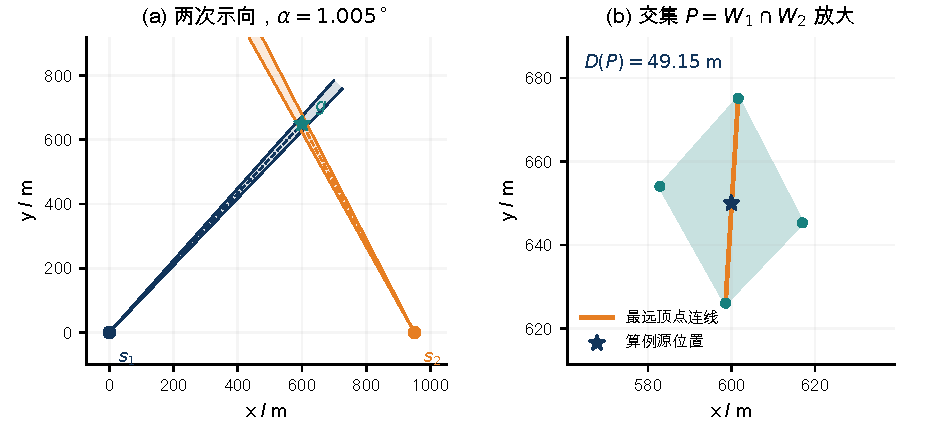
\includegraphics[width=\textwidth]{q1_wedge.pdf}
\caption{两次测向的楔形交会与定位区域放大图（自设几何算例）}
\label{fig:q1-wedge}
\end{figure}

\subsection{区域分类与顶点计算}
将式\eqref{eq:wedge}的约束统一记为$Ag\le b$。由于测向方向和检测位置不同，交集可能为空、无界或有界，具体按以下步骤判断。
\begin{enumerate}
\item 求解二维线性可行性问题。如果不存在满足全部约束的点，判为观测约束矛盾。
\item 对非空区域，分别计算$x$和$y$的最大值、最小值。四个值均有限时区域有界；否则区域直径为$+\infty$。
\item 对有界区域，枚举两条不平行边界直线的交点，保留满足所有半平面约束的点，去重后按凸边界排序。
\item 计算所有顶点对之间的欧氏距离，取最大值。若区域退化为线段，则取两端点距离；若退化为单点，则直径为0。
\end{enumerate}
设两条边界为$a_i^{\mathsf T}g=b_i$和$a_j^{\mathsf T}g=b_j$，记$\Delta=a_{ix}a_{jy}-a_{iy}a_{jx}$。当$\Delta\ne0$时，交点坐标为
\begin{equation}
x=\frac{b_i a_{jy}-a_{iy}b_j}{\Delta},\qquad
y=\frac{a_{ix}b_j-b_i a_{jx}}{\Delta}.
\end{equation}
每个交点需检查全部约束，朴素算法的时间复杂度为$O(m^3)$。本题一次局部定位使用的测向数量较少，该方法便于处理退化情形，计算量也较小。

\subsection{直径的顶点性质}
设非空有界区域$P=\conv\{v_1,\ldots,v_k\}$，则
\begin{equation}\label{eq:diameter}
D(P)=\max_{1\le i,j\le k}\norm{v_i-v_j}.
\end{equation}
证明如下。任意$p,q\in P$均可写成顶点的凸组合：$p=\sum_i a_i v_i$、$q=\sum_j b_j v_j$，其中系数非负且各自和为1。因此
\begin{align}
\norm{p-q}
&=\left\lVert\sum_{i,j}a_i b_j(v_i-v_j)\right\rVert\notag\\
&\le\sum_{i,j}a_i b_j\norm{v_i-v_j}
\le\max_{i,j}\norm{v_i-v_j}.
\end{align}
另一方面，各顶点本身属于$P$，最大顶点距离可以在区域内取到，故式\eqref{eq:diameter}成立。

\subsection{直径圆的覆盖能力}
区域的直径给出最大点间距离，但不直接给出覆盖整个区域的圆半径。取
\[
A=(0,0),\quad B=(36,0),\quad C=(18,18\sqrt3),
\]
形成边长36米的等边三角形。它的直径为36米，外接圆半径为
\begin{equation}
r=\frac{36}{\sqrt3}\approx20.784610\ \mathrm m>18\ \mathrm m.
\end{equation}
等边三角形的最小包围圆就是外接圆，因此任何直径36米的圆都不能覆盖其三个顶点。该例还说明，定位区域直径小于40米时，仍可能无法用20米光学半径一次覆盖。

为使反例对应题目的测向模型，依次沿三条有向边取单位方向$e_j$，令检测点为
\begin{equation}
S_j=V_j-\ell e_j,\qquad \ell=18\sqrt3\cot2^\circ-18.
\end{equation}
示向读数分别取$1^\circ$、$121^\circ$、$241^\circ$，理论误差为$\pm1^\circ$。各楔形的一条边沿三角形对应边，另一条经过对角顶点，交集恰为该三角形。检测点到三角形内各点的距离均小于1000米，符合接收条件。

\begin{figure}[htbp]\centering
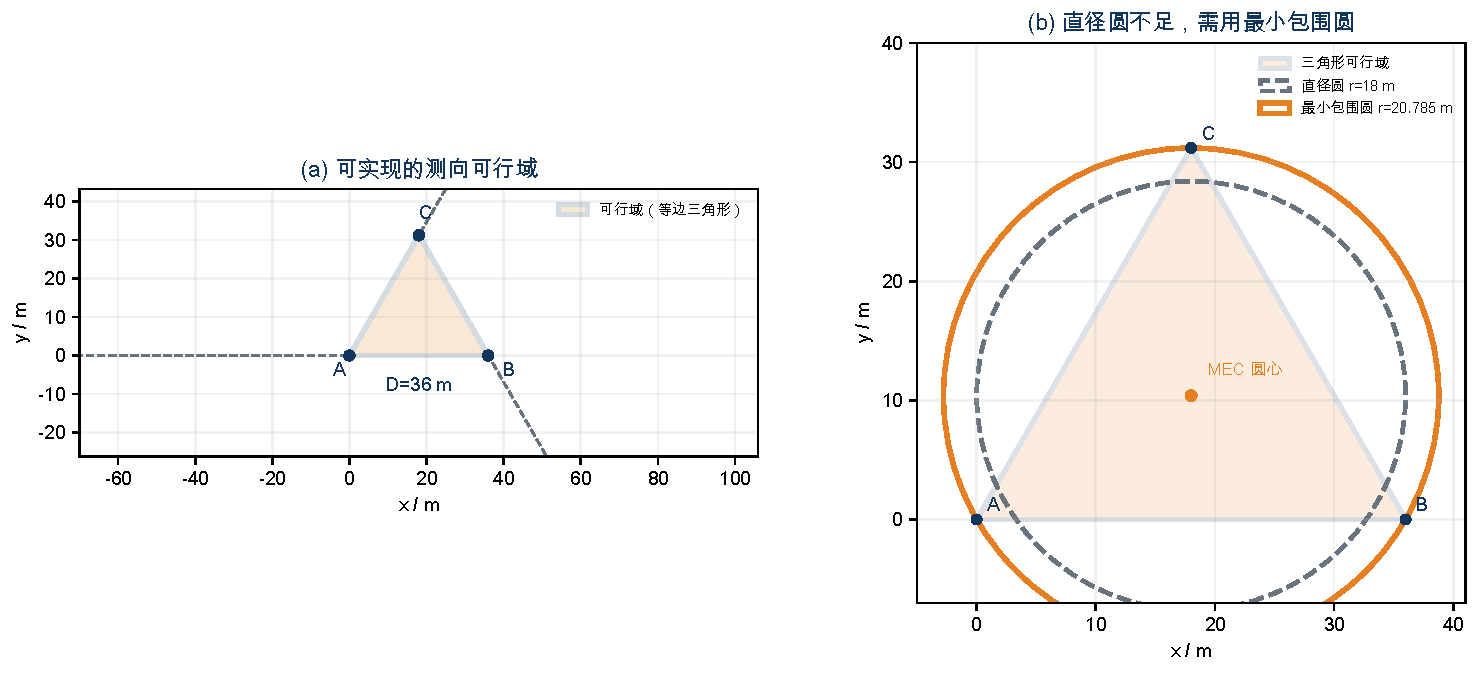
\includegraphics[width=\textwidth]{geometry.pdf}
\caption{三角形交会区域与两种覆盖圆的比较}
\label{fig:geometry}
\end{figure}

\subsection{最小包围圆与清除位置}
为了从位置区域选择清除点，定义
\begin{equation}\label{eq:mec}
r_*(P)=\min_z\max_{p\in P}\norm{p-z},\qquad
z_*(P)=\argmin_z\max_{p\in P}\norm{p-z}.
\end{equation}
圆盘是凸集，只要包含多边形全部顶点，便包含整个多边形。最小包围圆可由一个、两个或三个支持点确定，采用增量算法求解\cite{welzl}。在浮点计算中，对近共线点和最终半径保留向外余量。

平面凸区域满足
\begin{equation}\label{eq:jung}
\frac{D(P)}2\le r_*(P)\le\frac{D(P)}{\sqrt3}.
\end{equation}
左侧来自圆盘中任意两点距离不超过直径。若包围圆由两个点确定，则$r_*=D/2$；若由三个点确定，三个支持点中必有一对对应的圆心角不小于$120^\circ$，弦长不小于$\sqrt3r_*$，由此得到右侧。该平面包围圆界可由Jung定理得到\cite{jung}。

因此，$r_*(P)\le20$是存在一次全域清除位置的判断条件。若只使用直径，则$D(P)\le20\sqrt3$为充分条件，$D(P)>40$时不能一次覆盖；介于二者之间时需继续求最小包围圆。程序实际采用19.9米半径，并在选定点复算全部顶点距离。

\subsection{在线定位区域的更新}\label{subsec:online-region}
一次有效示向还说明源距检测点不超过1500米。沿示向轴取投影，得到线性约束
\begin{equation}
u(\theta_i)^{\mathsf T}(g-s_i)\le1500.
\end{equation}
设$A_{180}$为半径1800米圆域的外切正180边形，在线维护
\begin{equation}\label{eq:online-region}
P_c=A_{180}\cap\bigcap_{i\in I_c}
\left(W_i\cap\{g:u(\theta_i)^{\mathsf T}(g-s_i)\le1500\}\right).
\end{equation}
真实源初始位于$A_{180}$内，每条新增正观测约束也包含它，故逐步更新后仍有$g_c\in P_c$。外切近似的最大径向偏差为$1800(\sec(\pi/180)-1)<0.275$米。

新增一次观测时，采用逐边界裁剪的方式更新凸多边形，保留满足条件的顶点与边界交点\cite{sutherland}。若出现空域，说明观测或数值计算需要检查，当前频道不能据此记为无源。该表示同时提供局部测向的候选范围和清除位置判断。

\section{问题二：第二检测点的选择}
\subsection{交会几何对定位误差的影响}
移动单站定位通过改变观测位置，获得同一源在不同方向上的测向信息\cite{qin}；交叉定位中的方位误差还会随观测几何传播到位置结果\cite{li}。本问据此考察第二检测点的交会角和目标距离，位置估计仍采用前述有界误差可行域。


单次测向将源限制在长而窄的扇形内，但沿示向方向的距离仍不确定。设两次检测点到真实源的距离为$r_1,r_2$，视线夹角为$\beta$。对小角度误差线性化，位置扰动$\delta g$在每条视线法向$n_i$上满足
\begin{equation}
|n_i^{\mathsf T}\delta g|\le\alpha r_i.
\end{equation}
两条误差带的交集近似为平行四边形，面积为
\begin{equation}\label{eq:intersection-area}
A\approx\frac{4\alpha^2r_1r_2}{|\sin\beta|},
\end{equation}
其中$\alpha$以弧度计。固定距离时，交会角接近$90^\circ$有利于缩小误差；夹角接近$0^\circ$或$180^\circ$时，交会区域沿一个方向拉长。

第二点移动还会改变$r_2$，所以不能只按夹角选择。本文先限制第二点位于可接收区域，再通过楔形裁剪计算定位效果。式\eqref{eq:intersection-area}用于解释选点趋势，实际计算仍采用完整的角度约束。

图\ref{fig:q2-angle}固定两次测向距离，比较不同交会角对应的面积因子。两条视线接近平行时，误差面积迅速增大；接近直角时，该因子最小。实际选点还需同时考虑接收条件和移动距离。
\begin{figure}[htbp]\centering
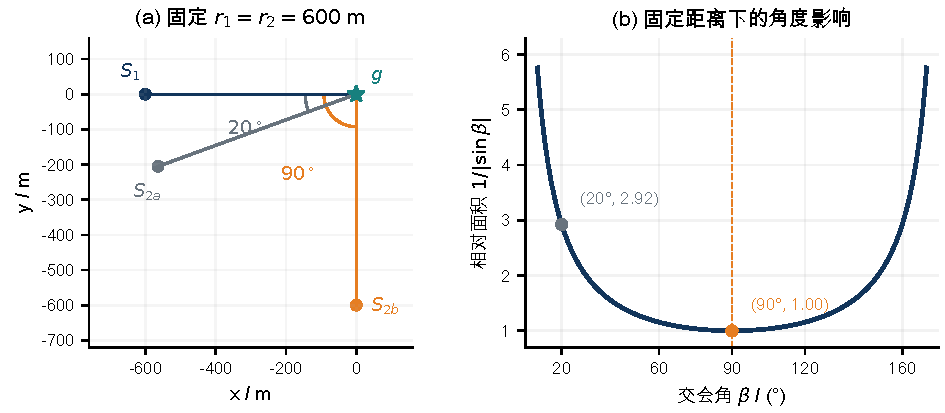
\includegraphics[width=\textwidth]{q2_angle.pdf}
\caption{固定测向距离时的交会角与相对误差面积}
\label{fig:q2-angle}
\end{figure}

\subsection{由首次接收得到的候选条件}
记首次检测点为$S_1$，读数方向为$u$，法向为$n$，第二点表示为
\begin{equation}
S_2=S_1+tu+bn.
\end{equation}
其中$t$是沿首次方向的前进距离，$b$是横向位移。设源到$S_1$的真实距离为$r$。由于首次已经接收到信号，未知接收半径至少满足
\begin{equation}
R_c\ge\max(1000,r).
\end{equation}
因此，对首次观测允许的所有源位置$g$，若第二点满足
\begin{equation}\label{eq:robust-reception}
\norm{S_2-g}\le\max(1000,\norm{g-S_1}),
\end{equation}
便能够再次接收信号。

令$u_\pm=u(\theta_1\pm\alpha)$，把首次可行位置放宽为$r\in[0,1500]$、角差$\varphi\in[-\alpha,\alpha]$的扇形，得到三圆交候选域
\begin{equation}\label{eq:lens}
\mathcal C=S_1+\left[B(0,1000)\cap B(1000u_-,1000)
\cap B(1000u_+,1000)\right].
\end{equation}
该候选域使用接收半径下界和首次接收事实，不需要估计目标的具体距离。

\subsection{三圆交条件的推导}
取$q=S_2-S_1$。从$r=0$及$r=1000,\varphi=\pm\alpha$这三种位置，可得式(\ref{eq:lens})中的三个圆盘约束。下面验证这些约束对整个放宽扇形均适用。

由$\norm{q-1000u_\pm}\le1000$，展开可得
\begin{equation}\label{eq:lens-projection}
q^{\mathsf T}u_\pm\ge\frac{\norm q^2}{2000}\ge0.
\end{equation}
对于两端方向之间的小圆弧，投影$q^{\mathsf T}u_\varphi$的最小值位于端点，因而也满足式\eqref{eq:lens-projection}。

当$0\le r\le1000$时，$\norm{q-r u_\varphi}$是$r$的凸函数。$r=0$和$r=1000$两端的值均不超过1000，内部也不超过1000。当$r\ge1000$时，
\begin{equation}
\norm{q-r u_\varphi}^2-r^2
=\norm q^2-2r q^{\mathsf T}u_\varphi\le0.
\end{equation}
于是源到第二点的距离不超过$\max(1000,r)$，式(\ref{eq:robust-reception})成立。实际源位置还受目标圆域约束，采用放宽扇形可使选点条件保持统一。

\subsection{候选点生成与排序}
在以首次示向方向为$t$轴的坐标系中，三圆交写成
\begin{equation}\label{eq:lens-coordinates}
\left\{\begin{aligned}
t^2+b^2&\le1000^2,\\
(t-1000\cos\alpha)^2+(b-1000\sin\alpha)^2&\le1000^2,\\
(t-1000\cos\alpha)^2+(b+1000\sin\alpha)^2&\le1000^2.
\end{aligned}\right.
\end{equation}
给定$t$后，横向边界为
\begin{equation}\label{eq:bmax}
 b_{\max}(t)=\min\left\{\sqrt{1000^2-t^2},
 \sqrt{1000^2-(t-1000\cos\alpha)^2}-1000\sin\alpha\right\}.
\end{equation}
根号有定义且$b_{\max}\ge0$时，取$0<t<1000$和$0<|b|\le b_{\max}(t)$，形成首次方向两侧的候选区域。计算中设置
\begin{equation}
\begin{aligned}
t&\in\{125,250,375,500,625,750,875\}\ \mathrm m,\\
b&=\pm\kappa b_{\max}(t),\qquad
\kappa\in\{1/4,1/2,3/4\},
\end{aligned}
\end{equation}
共得到42个候选点。

对每个候选点，枚举当前区域中的样本源位置及第二次测向误差，计算新楔形与当前区域的交集，再求最小包围圆半径。以样本中的最大半径作为该点的评分，优先选择评分较小的点；几何效果接近时再比较本步移动费用。这使候选点的接收条件由三圆交确定，定位效果由实际交会计算得到。

\begin{figure}[htbp]\centering
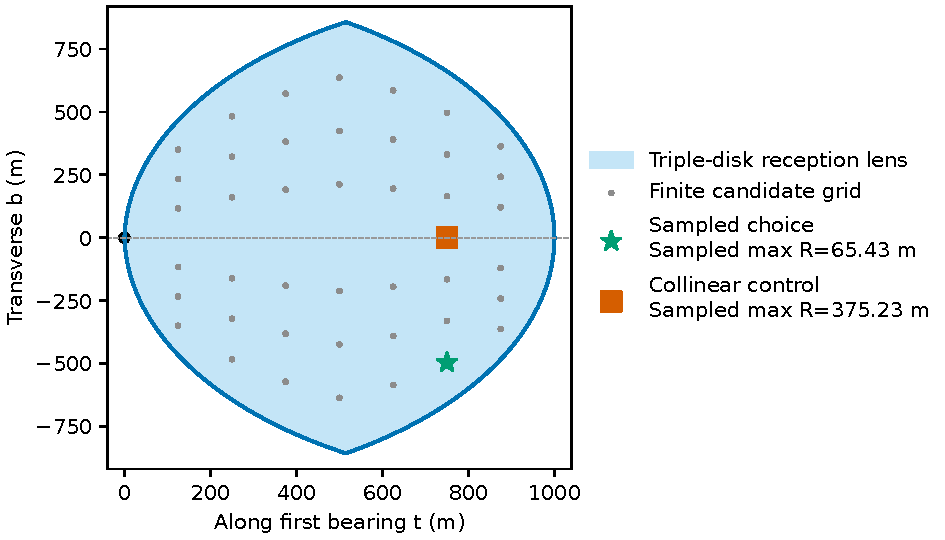
\includegraphics[width=\textwidth]{q2_lens.pdf}
\caption{第二检测点的接收区域与横向候选}
\label{fig:lens}
\end{figure}

\subsection{算例结果与分析}
令$S_1=(0,0)$、$\theta_1=0$，设置60个径向位置、3个首次真实角差和3个第二次测向误差。由此比较42个候选点与共线对照，结果见表\ref{tab:q2-example}。
\begin{table}[H]\centering\small
\caption{第二检测点算例结果}\label{tab:q2-example}
\begin{tabular}{lrrr}\toprule
测点类型 & 坐标/米 & 采样最坏半径/米 & 移动与检测/秒\\\midrule
横向候选 & $(750,-496.078)$ & \QTwoRadius & \QTwoCost\\
共线对照 & $(750,0)$ & \QTwoControlRadius & \QTwoControlCost\\\bottomrule
\end{tabular}
\end{table}
横向候选增加约\QTwoExtraCost{}秒的本步费用，但将样本中的最坏包围半径从\QTwoControlRadius{}米减至\QTwoRadius{}米，说明横向基线对径向误差具有明显改善作用。该半径仍大于20米，后续还需继续测向或实施光学搜索。此例给出离散候选中的选择结果，在线多源搜索则采用中心横向测点。

\section{问题三：全向干扰源的搜索、定位与清除}
\subsection{七点扫描骨架}
问题三所有源均全向发射。只要检测点的1000米接收圆盘覆盖整个目标圆域，所有存在的频道便能在有限次扫描中至少收到一次信号。选取原点与半径$d$的正六边形环：
\begin{equation}\label{eq:ring-points}
p_0=(0,0),\qquad p_{k+1}=d\,u(k\pi/3),\quad k=0,\ldots,5.
\end{equation}
这些点只规定全域扫描位置，实际访问顺序随已发现源和机器狗当前位置调整。

为计算覆盖半径，设任意源$g=r u(\theta)$。总能选择一个环点，使其极角与源相差不超过$\pi/6$。在半径$r$的圆周上，距最近检测点的最坏距离为
\begin{equation}\label{eq:ring-envelope}
f_d(r)=\min\left\{r,\sqrt{r^2+d^2-\sqrt3dr}\right\}.
\end{equation}
第一项对应原点，第二项对应相邻环点的角平分线。两项在$r=d/\sqrt3$处相等；在此之前原点更近，之后环点更近。后一项的平方为凸二次函数，故其最大值在区间端点取到。

在$1200\le d\le900\sqrt3$的构型范围内，全域覆盖半径为
\begin{equation}\label{eq:ring-radius}
\rho(d)=\max\left\{\frac d{\sqrt3},
\sqrt{R_0^2+d^2-\sqrt3R_0d}\right\}.
\end{equation}
两个候选最大值分别出现在圆内的等距点和圆周的角平分线处，因而式\eqref{eq:ring-radius}也给出了该构型的实际最坏距离。

\subsection{环半径与行程的选择}
当$d=900\sqrt3$时，式\eqref{eq:ring-radius}两项均为900米。向内收缩检测环能够缩短行程，同时会增大圆周处的最坏接收距离。选取$d=1200$米，可得
\begin{equation}\label{eq:ring-margin}
\begin{aligned}
\rho(1200)&=\sqrt{1800^2+1200^2-\sqrt3\cdot1800\cdot1200}\\
&\approx968.901572\ \mathrm m,\\
1000-\rho(1200)&\approx31.098428\ \mathrm m.
\end{aligned}
\end{equation}
因此七点骨架在缩短行程后仍保留约31.10米距离余量。若理想检测点与实际位置相差不超过$\eta$米，由三角不等式，最坏距离增加量不超过$\eta$。

从原点出发访问六个环点，首段至少为$d$，任意两个不同环点的距离不小于$d$。沿圆周依次访问恰达到
\begin{equation}\label{eq:ring-tour}
L_{\mathrm{ring}}^{\min}=6d.
\end{equation}
故完整骨架路线由$5400\sqrt3$米缩短为7200米。这个行程只包含骨架访问，完整任务还需加上定位支线和操作费用。

\begin{figure}[htbp]\centering
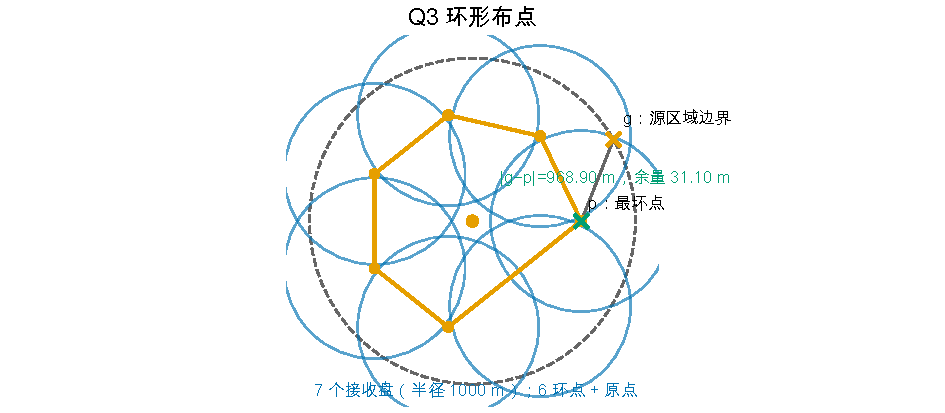
\includegraphics[width=0.76\textwidth]{competition_ring.pdf}
\caption{七点环的接收覆盖及圆周最坏位置}
\label{fig:ring}
\end{figure}

七点方案有明确的覆盖依据。作为点数比较，在900米覆盖要求下，单个接收盘对半径1800米圆周的交弧宽度最多为$60^\circ$。若仅用六盘覆盖整条圆周，六盘必须全部取到最大弧宽，并按正六边形排列；此时原点仍未被覆盖，还需增加一个中心盘。这个七点下界针对900米接收盘，1000米物理下界下的任意布局不在该下界的结论范围内。

图\ref{fig:q3-tradeoff}将式\eqref{eq:ring-radius}和式\eqref{eq:ring-tour}放在同一参数范围内比较。扩大环半径能够缩短最坏接收距离，但同时增加骨架行程；1200米环在保留接收余量的同时采用较短的扫描路线。
\begin{figure}[htbp]\centering
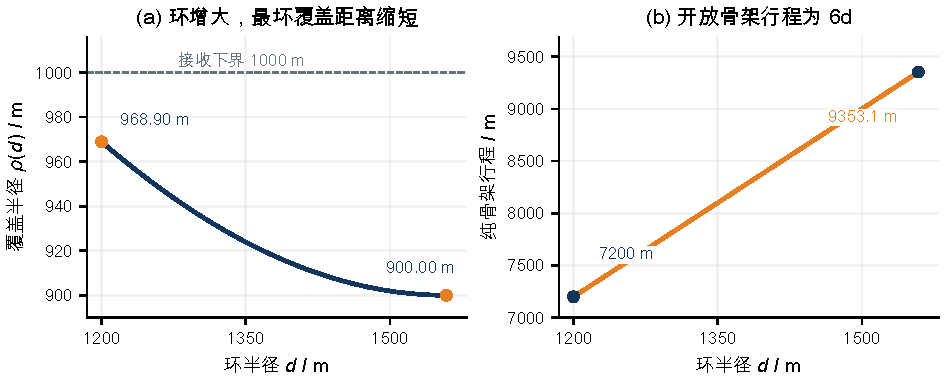
\includegraphics[width=\textwidth]{q3_tradeoff.pdf}
\caption{七点环覆盖距离与开放骨架行程的变化（不含定位及操作费用）}
\label{fig:q3-tradeoff}
\end{figure}

\subsection{扫描任务与定位任务的联合排序}
设当前位置为$q$。待执行任务分为两类：尚未完成的骨架扫描点，以及已经发现但未清除的源。扫描点用实际坐标表示，源任务用当前可行域的最小包围圆中心$z_c$表示。为统一符号，记各任务坐标为$z_j$，扫描任务半径为0，源任务半径为$r_j$。

对任务排列$\pi$，构造开放路线评分
\begin{equation}\label{eq:route-proxy}
J_\gamma(\pi)=\norm{q-z_{\pi_1}}+
\sum_{j=1}^{n-1}\norm{z_{\pi_{j+1}}-z_{\pi_j}}+\gamma r_{\pi_1}.
\end{equation}
问题三取$\gamma=0$，按任务中心之间的行程排序。基准策略refined先用最近插入法形成完整排列\cite{rosenkrantz}，再进行有界2-opt改进\cite{croes}：反转一段连续路线，若首尾连接费用下降则接受。每轮只执行得到的第一项任务，执行后重新计算位置区域和剩余任务。

扫描点与源任务保持各自身份，即使坐标相同也不合并。这样既可减少定位结束后返回原扫描点的绕行，也能保留未知频道的扫描义务。由于后续观测可能改变目标中心和清除终点，式\eqref{eq:route-proxy}作为当前任务排序依据，实际费用仍按式\eqref{eq:time}累计。

\subsection{逐频道扫描规则}
到达一个骨架点后，优先检测测向机当前频道，再依频道编号检测其余频道。已清除频道跳过；未知频道必须检测；已有有效示向且尚未清除的频道作为独立定位任务，不再要求在每个骨架点重复检测。

每次局部清除结束后，机器狗还可以在当前位置为其他已知频道补充测向。当该频道的包围半径大于19.9米、当前位置到其包围圆的最短距离不超过1500米，且未在完全相同坐标测过时，进行一次停靠共享检测。它不增加移动距离，但照常计入检测和换频费用。

\subsection{局部定位与清除步骤}\label{subsec:localization}
对已发现频道$c$，根据式\eqref{eq:online-region}维护位置多边形，计算其包围圆$B(z,r)$。局部过程先检查能否直接清除，再决定是否继续测向。
\begin{enumerate}
\item 若当前位置到所有顶点距离不超过19.9米，则原地清除；否则若$r\le19.9$米，则前往$z$清除。
\item 若$19.9<r\le38$米，先在$z$作一次光学尝试。成功即结束该频道；失败后进入矩形光学覆盖。
\item 若区域仍较大，取最近一次有效测向点$s^+$，令
\[
e=\frac{z-s^+}{\norm{z-s^+}},\qquad n=(-e_y,e_x),
\]
在中心两侧设置候选点
\begin{equation}\label{eq:flank}
p_\pm=z\pm\delta n,\qquad
\delta=\min\{120,\max\{25,0.22r\}\}\ \mathrm m.
\end{equation}
从未重复测过、未尝试失败的候选中选较近者。
\item 有效示向继续裁剪$P_c$；返回近源则原地清除。若无信号，在该点先作一次光学尝试，失败后再决定下一测点。问题三累计两次无信号后转入光学覆盖。
\item 每次局部定位最多使用6个新测向点；达到上限、没有新候选或中心方向退化时，转入光学覆盖。
\end{enumerate}
其中38米是试清与继续测向之间的切换阈值，19.9米是整个区域的一次清除判据。中心横向规则借助新的交会角缩小可行域，计算量小；它不要求每个在线测点都位于问题二的三圆交中，因此保留无信号处理分支。

\subsection{矩形光学覆盖}
当测向收缩不足时，取$P_c$的一条直径方向作为局部$x$轴，计算包含整个多边形的投影矩形$[x_-,x_+]\times[y_-,y_+]$。设有效网格半径为$\rho_o=19.9-\varepsilon$，取单元边长上限$h=\sqrt2\rho_o$，划分数为
\begin{equation}
N_x=\max\left(1,\left\lceil\frac{x_+-x_-}{h}\right\rceil\right),\qquad
N_y=\max\left(1,\left\lceil\frac{y_+-y_-}{h}\right\rceil\right).
\end{equation}
第$(i,j)$格中心为
\begin{equation}
a_{ij}=\left(x_-+\frac{i+1/2}{N_x}(x_+-x_-),\quad
 y_-+\frac{j+1/2}{N_y}(y_+-y_-)\right).
\end{equation}
任一单元的半对角线不超过$h/\sqrt2=\rho_o$，故半径19.9米的圆盘能够覆盖整个单元。由此得到
\begin{equation}\label{eq:optical-cover}
P_c\subseteq\bigcup_{i=0}^{N_x-1}\bigcup_{j=0}^{N_y-1}B(a_{ij},19.9).
\end{equation}
这些圆盘的并集覆盖整个区域，而非只覆盖多边形顶点。逐个中心并不需要覆盖整个$P_c$，因此部分清除失败属于正常搜索过程。

区域分解后逐行往复访问，是机器人覆盖规划中的常用思路\cite{galceran}。本文按蛇形排列访问各中心，再将序列循环移位，使首点靠近当前位置。真实源在某个单元内，遍历过程中至少有一个中心落在它的清除范围内，收到成功反馈后立即结束该频道。

\begin{figure}[htbp]\centering
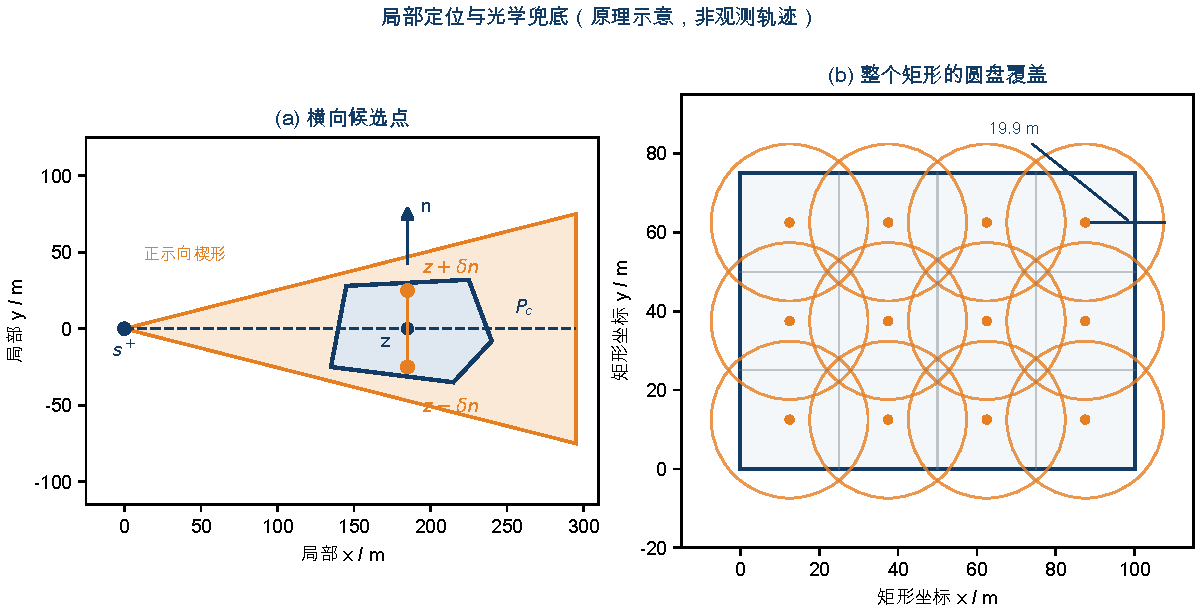
\includegraphics[width=\textwidth]{competition_localize.pdf}
\caption{中心横向测点与矩形光学覆盖示意}
\label{fig:localization}
\end{figure}

\subsection{全向负观测与安全接近}
在基准策略上，增强策略field利用全向无信号信息缩小位置区域。若某频道尚有源，在位置$s$检测无信号，则有$\norm{g_c-s}>1000$。直接从凸多边形中减去圆盘会产生非凸区域，因此采用凸外包近似。

在1000米圆盘内部构造正十六边形
\begin{equation}
Q_s=\conv\left\{s+1000\cos\frac\pi{16}\,
 u\left(\frac{2j\pi}{16}\right):j=0,\ldots,15\right\}.
\end{equation}
令$H_j^{\mathrm{out}}$为其第$j$条边的闭外侧半平面，更新为
\begin{equation}\label{eq:negative}
P_c^+=\conv\left(\bigcup_{j=0}^{15}(P_c\cap H_j^{\mathrm{out}})\right).
\end{equation}
由于$Q_s$严格位于接收圆盘内，圆盘外的真实源一定落在至少一个保留半平面中；取凸包仍包含它，且$P_c^+\subseteq P_c$。算法保存发现源之前的无信号位置，建立轨迹后也可应用这些信息。

field还在已经满足全域清除条件时缩短接入距离。设原计划清除点为$a$，当前位置为$q$，沿$u=(q-a)/\norm{q-a}$取$a'=a+tu$。对每个顶点$v$要求
\begin{equation}
t^2+2(a-v)^{\mathsf T}u\,t+\norm{a-v}^2-19.9^2\le0.
\end{equation}
以所有顶点给出的上界和$\norm{q-a}$中的最小值确定$t$，再复验新点到全部顶点的距离。该操作只改变已确定清除点的接近位置；基准refined不使用此项优化。

\subsection{频道状态与停止条件}
对每个频道记录四种状态：未确定$U$、已发现$D$、已清除$C$和完成覆盖后无源$A$。设七点骨架为$V$，频道$c$已经实际检测的骨架索引为$V_c$。只有从未发现且$V_c=V$的频道，才可以由全无信号转为$A$；已经发现的频道由清除成功转为$C$。

停止条件为
\begin{equation}\label{eq:stop}
\left[\forall c,\ \mathrm{state}_c\in\{C,A\}\right]
\quad\text{或}\quad
\left[\#\{c:\mathrm{state}_c=C\}=16\right].
\end{equation}
第一种情况由七点全域覆盖排除了未发现源，第二种情况使用题给源数上界。已清除10个源或当前没有定位任务时，仍继续完成剩余未知频道的扫描。

\section{问题四：定向干扰源的搜索、定位与清除}
对定向源，距离足够近还需满足式(\ref{eq:visibility})的前向条件。圆周源若朝圆外发射，所有严格位于圆内的点都可能在发射背面。因此在目标圆域外增加一层检测点，并与内部点形成连续剖分。

取内环半径$a=940$米、外环半径$b=1870$米，定义
\begin{equation}\label{eq:polar-points}
\begin{aligned}
O&=(0,0),\\
I_k&=a\,u(k\pi/6),\\
E_k&=b\,u(k\pi/6+\pi/12),\qquad k=0,\ldots,11.
\end{aligned}
\end{equation}
内外环相邻点分别相差$30^\circ$，两环错开$15^\circ$。点集包括原点、12个内环点和12个外环点，共25个位置。外环点虽超出源所在圆域，但属于机器狗允许访问的位置。

\subsection{三角剖分及距离界}
以下下标按模12计算，构造
\begin{equation}\label{eq:triangulation}
\begin{aligned}
T_k^{(1)}&=\conv\{O,I_k,I_{k+1}\},\\
T_k^{(2)}&=\conv\{I_k,E_k,I_{k+1}\},\\
T_k^{(3)}&=\conv\{I_{k+1},E_k,E_{k+1}\}.
\end{aligned}
\end{equation}
第一类三角形填满内十二边形，后两类填满内外两环之间的带状区域。连接边位于对应的$15^\circ$扇区内，且$a<b\cos(\pi/12)$，因此各三角形内部不交叉，共同组成外正十二边形$H=\conv\{E_k\}$。

记$c=\cos(\pi/12)$、$s=\sin(\pi/12)$，剖分中仅有四类边长：
\begin{equation}\label{eq:edge-lengths}
\ell_0=a,\quad\ell_I=2as,\quad\ell_E=2bs,\quad
\ell_{IE}=\sqrt{a^2+b^2-2abc}.
\end{equation}
利用$c>0.9659$、$s<0.259$，有
\begin{align}
bc&>1806.233>1805,\notag\\
\ell_0&=940<993,\qquad \ell_I<486.92<993,\notag\\
\ell_E&<968.66<993,\notag\\
\ell_{IE}^2&<984781.96<993^2.
\end{align}
于是$H$包含半径1805米的圆盘，每个三角形直径小于993米。这两个界分别保证辅助点位于剖分内，并限制辅助点到三角形顶点的距离。

\subsection{任意发射方向的覆盖证明}
任取源位置$g\in\disk$与发射单位向量$n$，沿发射方向引入辅助点
\begin{equation}\label{eq:helper}
h=g+5n.
\end{equation}
因$\norm g\le1800$，有$\norm h\le1805$，所以$h$属于剖分中的某个闭三角形$T$。将其表示为顶点的重心组合
\[
h=\sum_{i=1}^3\lambda_i v_i,\qquad \lambda_i\ge0,\quad\sum_i\lambda_i=1,
\]
沿$n$方向投影得到
\begin{equation}
\sum_i\lambda_i n^{\mathsf T}(v_i-g)
=n^{\mathsf T}(h-g)=5.
\end{equation}
至少存在一个顶点$v$使$n^{\mathsf T}(v-g)\ge5$。同时$v,h$位于同一三角形，故
\begin{equation}
\norm{v-g}\le\norm{v-h}+\norm{h-g}<993+5=998.
\end{equation}
若实际检测点$v'$与理想点相差不超过1米，则
\begin{equation}\label{eq:direction-margin}
n^{\mathsf T}(v'-g)\ge4\ \mathrm m,\qquad
\norm{v'-g}<999\ \mathrm m.
\end{equation}
因此所选点严格位于发射前方，且距源小于最小接收半径1000米。该证明对任意$g,n$均成立，源在圆周、辅助点落在边或顶点上时也适用。

\begin{figure}[htbp]\centering
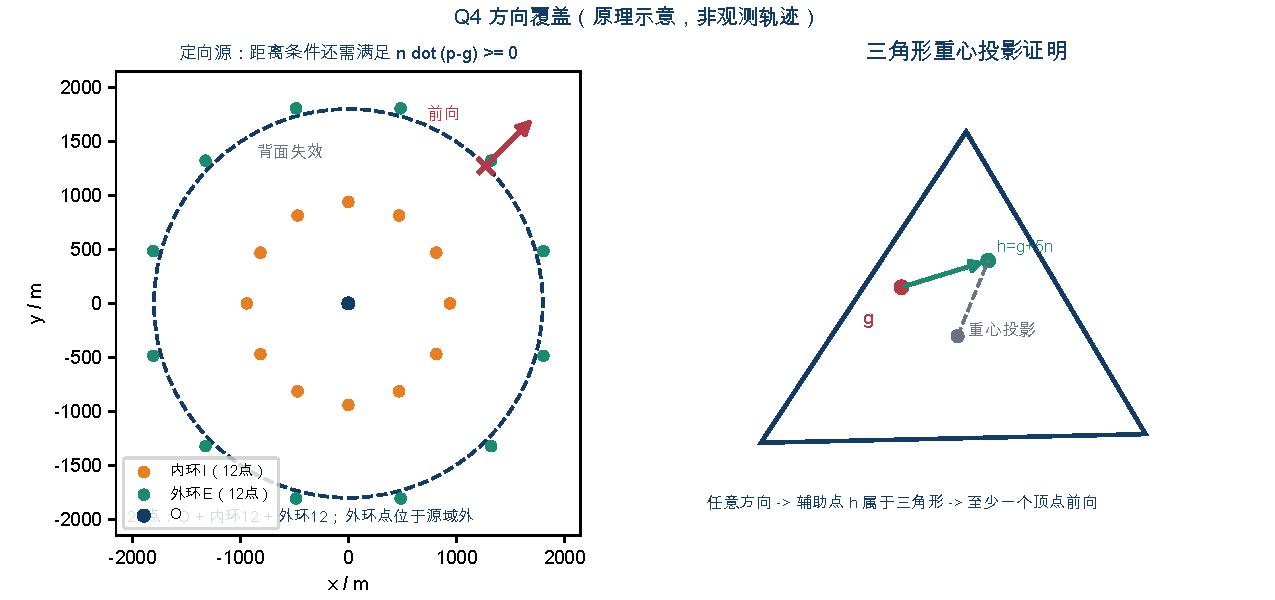
\includegraphics[width=\textwidth]{competition_direction.pdf}
\caption{双环检测点与前向投影的几何关系}
\label{fig:direction}
\end{figure}

辅助点仅用于证明，机器狗不需要估计源的发射方向或访问$h$。1米位置余量表示坐标计算、舍入和停靠偏差的总量。方向覆盖的实际实现仍按式\eqref{eq:polar-points}给出的25个固定点执行。

\subsection{骨架路径与扫描次数}
一条访问25点的开放路线为
\[
O,I_0,I_1,\ldots,I_{11},E_{11},E_{10},\ldots,E_0.
\]
对应长度为
\begin{equation}
L_{25}=a+22(a+b)\sin\frac\pi{12}
+\sqrt{a^2+b^2-2ab\cos\frac\pi{12}}
\approx17932.51\ \mathrm m.
\end{equation}
它用于说明骨架能够连成有限路线，实际顺序由任务调度决定。相较31点骨架，若20个频道均完成全部扫描，25点方案少120次检测，对应检测项少600秒；实际任务会随频道清除和已知频道补测筛选而改变次数。

图\ref{fig:q4-route}比较上述可行骨架路线与已有的refined本地模拟轨迹。右图取种子20260910的单局记录，只按已执行动作连接位置，标出的清除位置不是源坐标真值。两条路线的区别反映了局部定位支线与在线任务重排，不能把纯骨架长度直接当作完整任务行程。
\begin{figure}[htbp]\centering
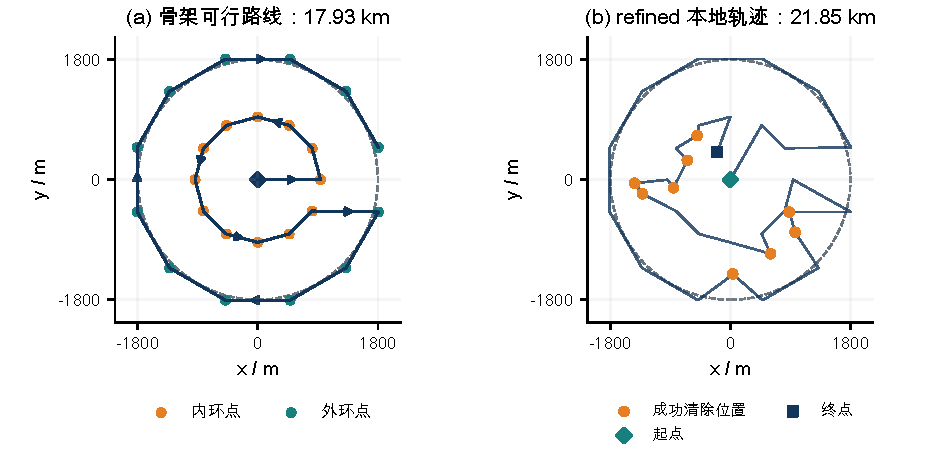
\includegraphics[width=\textwidth]{q4_route.pdf}
\caption{Q4双环骨架路线与本地模拟轨迹（右图为refined，非正式测试轨迹）}
\label{fig:q4-route}
\end{figure}

\subsection{路线组合与补测筛选}
问题四采用field路线组合，对式\eqref{eq:route-proxy}取$\gamma=1$。当首项为不确定区域较大的源任务时，半径项增加其评分；当首项是扫描点时，该项为0。由此兼顾到达距离和当前定位范围。

候选路线包括原最近插入及有界2-opt路线、全局最便宜插入路线，以及以两个不同首任务起步的近邻路线。对每个不同初解，最多进行$\min(n,12)$轮改进，检查连续区间反转和单点搬移两类操作，再从全部完整排列中选择评分最小者。

保留原路线使组合评分不高于原控制路线，但观测和清除终点会在执行后变化，最终收益由总虚拟时间评价。构建距离矩阵需要$O(n^2)$空间，有界搜索的保守时间上界为$O(n^3)$。

骨架扫描采用有用补测规则。未知频道仍必须检测；对已有轨迹的频道，只有当
\begin{equation}\label{eq:useful}
r_c>19.9,\qquad \norm{p-z_c}-r_c\le1500
\end{equation}
时继续补测。若区域已足够小，可直接清除；若整个包围圆都超过接收上限，继续测向没有价值。跳过已知频道不会形成无源记录，该频道仍需成功清除。

field在局部定位前还可进行一次原地预检测。触发条件为：该频道尚未使用预检测机会，当前位置未测过该频道，$r_c>38$，且$\norm{q-z_c}-r_c\le1500$。这一次检测位于原有6次测向之外，照常计入检测与换频费用。它有机会在移动前收缩区域，减少后续偏移距离。

\subsection{失信号恢复}
定向源在新位置可能落到发射背面。为继续利用最后一次有效测向，设该测点为$s^+$，由其指向当前包围圆中心的方向为$e$，法向为$n$。将失败测点写成
\[
p^--s^+=a e+b n,
\]
恢复点取
\begin{equation}\label{eq:recovery}
p^{\mathrm{next}}=s^++\frac12(ae-bn).
\end{equation}
该操作把横向分量反向，并将相对$s^+$的距离缩短一半。新的有效测向出现后，更新$s^+$和方向轴；若仍无信号，则在6次测向预算内继续恢复，之后转为矩形光学覆盖。

Q4的无信号信息不用于整圆盘位置排除，因为发射背面的源仍可能位于1000米以内。Q4也不启用安全近侧清除项，清除位置沿用基准局部过程。光学搜索按式\eqref{eq:optical-cover}的圆盘并集覆盖区域，每个覆盖中心只负责对应小单元；遍历全部中心后即可覆盖整个位置域，不要求每个中心单独覆盖整个$P_c$。

\subsection{整体执行与有限终止}
问题四以$V=\{0,\ldots,24\}$替换问题三的七点索引，状态转移和停止条件仍用式\eqref{eq:stop}。若未知频道在全部25点都无信号，与任意方向覆盖结论矛盾的源便不存在；已发现频道只有收到成功清除反馈才完成。

每次完整骨架扫描结束后，不再返回已经完成的扫描点。每个正常局部任务清除一个新源，最多有16个；每个局部任务至多一次预检测和6次新测向，随后进入有限光学网格。因此在正常反馈和误差条件下，扫描与定位均能在有限动作内完成。

\begin{table}[H]\centering\small
\caption{两类问题的主要执行规则}
\begin{tabular}{p{3cm}p{5.1cm}p{5.1cm}}\toprule
环节 & 问题三 & 问题四\\\midrule
发现骨架 & 原点及1200米六点环 & 原点及940/1870米错相双环\\
任务评分 & 首项半径权重$\gamma=0$ & 首项半径权重$\gamma=1$\\
已知频道骨架补测 & 跳过，保留独立定位任务 & 满足式\eqref{eq:useful}时补测\\
无信号处理 & field可用负观测凸外包 & 保留位置域，回退恢复\\
局部结束 & 直接清除或矩形覆盖 & 直接清除或矩形覆盖\\
全局停止 & 全频道完成或16源清除 & 全频道完成或16源清除\\\bottomrule
\end{tabular}
\end{table}

\subsection{算法执行流程}
将上述过程整理为图\ref{fig:whole-algorithm}。机器狗先建立扫描点和20个频道的状态记录，再检查是否满足停止条件；若尚有任务，就依据当前位置重排任务。选中扫描点时，完成该点的必要频道检测；选中源任务时，调用局部测向和光学清除过程。两条分支都回到状态更新，不要求机器人返回先前扫描点。
\begin{figure}[htbp]\centering
\begin{tikzpicture}[>=Stealth,node distance=8mm and 16mm,
process/.style={draw,rounded corners=2pt,align=center,text width=47mm,minimum height=11mm,font=\small},
judge/.style={draw,diamond,aspect=3,align=center,inner sep=1pt,font=\small}]
\node[process] (start) {初始化扫描点与频道状态};
\node[judge,below=of start] (stop) {满足停止条件？};
\node[process,right=17mm of stop,text width=17mm] (end) {结束};
\node[process,below=of stop] (choose) {按当前位置重排剩余任务};
\node[process,below left=10mm and 2mm of choose] (scan) {骨架任务\\检测未知及有用频道};
\node[process,below right=10mm and 2mm of choose] (locate) {源任务\\有限测向与光学清除};
\node[process,below=27mm of choose] (update) {更新位置域、扫描记录与清除状态};
\draw[->] (start)--(stop);
\draw[->] (stop)--node[above]{是}(end);
\draw[->] (stop)--node[right]{否}(choose);
\draw[->] (choose)-|(scan);
\draw[->] (choose)-|(locate);
\draw[->] (scan)|-(update);
\draw[->] (locate)|-(update);
\draw[->] (update.south)--++(0,-7mm)--++(-69mm,0)|-(stop.west);
\end{tikzpicture}
\caption{扫描与定位交替进行的任务执行流程}
\label{fig:whole-algorithm}
\end{figure}

光学后备的搜索规模还可以由单次测向范围估计。沿最近一次有效示向轴，位置域的纵向长度不超过约1500米，横向宽度不超过$2\times1500\tan(1.005^\circ)<53$米。转到直径对齐坐标后，可用长小于1501米、宽小于106米的矩形包围；按第\ref{subsec:localization}节的网格边长划分，至多需要
\begin{equation}
N_{\rm cell}\le\left\lceil\frac{1501}{\sqrt2(19.9-\varepsilon)}\right\rceil
\left\lceil\frac{106}{\sqrt2(19.9-\varepsilon)}\right\rceil
=54\times4=216
\end{equation}
个中心，其中$\varepsilon$取实现中的微小向内余量。实际可行域通常经过多次裁剪，所需网格少于此上界。

\subsection{算法终止性与时间上界}\label{subsec:termination-bound}
设接口正常响应，测向误差满足题设条件。问题三、四分别有7个和25个骨架任务，完成后即从任务集合中删除。对已发现频道，局部过程至多进行6次测向，随后直接清除或进入至多216个中心的光学覆盖。由于真实源始终位于覆盖区域内，遍历全部中心前必有一次清除成功。因此，每轮调度至少完成一个骨架任务或清除一个新源，已完成任务不再加入；源数又不超过16，算法最终满足式\eqref{eq:stop}。

按较大的25点骨架计，骨架检测至多$25\times20$次；停靠共享只在局部任务结束后进行，至多16轮，每轮至多检测16个已知频道；局部测向和field预检测分别至多$16\times6$次和16次。由此有
\begin{equation}\label{eq:measurement-bound}
M\le25\times20+16\times16+16\times6+16=868\le1228.
\end{equation}
下文按$M\le1228$统一估计检测费用。每源计入216次网格清除、至多6次无信号后试清、一次小区域试清，并为其他位置的成功清除留一次余量，则清除调用总数满足
\begin{equation}\label{eq:clear-call-bound}
C=F+K\le16(216+6+1+1)=3584.
\end{equation}

时间上界还需计入行程。由前述位置域尺寸，包围圆中心距最近正测点小于1501米，横向偏移不超过120米，故首个候选测点距该正测点小于$\sqrt{1501^2+120^2}<1506$米。恢复操作只缩短这一距离，因而局部测点距源小于$1500+1506=3006$米，距原点小于4806米。骨架点和已清除源的终点距原点均小于2620米，于是每段骨架抵达、局部任务接入和两次测向间的行程可分别放宽为5240、7500和6020米。圆心清除与光学搜索的接入段各不超过4520米；矩形内蛇形路径连同一次循环移位跳跃小于7570米。
\begin{equation}\label{eq:travel-bound}
\begin{aligned}
L&\le25\times5240+
16(7500+5\times6020+2\times4520+7570)\\
&=998360\ \mathrm m.
\end{aligned}
\end{equation}
每次检测至多附带一次换频，每次清除至多耗时5秒。将上述上界代入计时模型，得到
\begin{equation}\label{eq:virtual-time-bound}
\begin{aligned}
T&\le\frac L5+6M+5C\\
&\le\frac{998360}{5}+6\times1228+5\times3584\\
&=224960\ \mathrm s<100\times3600\ \mathrm s.
\end{aligned}
\end{equation}
该估计将各阶段的最大费用相加，用于核对100小时虚拟时间限制；现实运行期限仍按接口返回的剩余时间执行。

\section{数值试验与结果分析}\label{sec:experiments}
为了比较任务调度和局部机制，在同一合成世界上分别运行各配置。常规世界中，源数在10至16之间离散均匀取值，频道无放回抽样，位置在半径1800米圆域内按面积均匀生成，接收半径在1000至1500米之间均匀生成。问题三全部为全向源；问题四设置混合源，定向源的方向均匀生成。

误差场采用三种设置：有界双正弦平滑场、位置哈希取$\pm1^\circ$的端点场、位置哈希在$[-1^\circ,1^\circ]$中取值的误差场。同一位置的误差固定，读数保留两位小数。上述设置用于构造可重复测试场景，不作为官方生成器的分布估计。

开发阶段每题使用150个世界比较候选配置，之后固定参数，在每题1000个新世界上进行主比较。Q3列出refined、仅路线增强、路线与信息、完整field四组；Q4比较refined与field两组，主组共6000次策略执行。另进行边界情形和替代误差测试，合计9400次执行，各组分别统计。

\subsection{主组比较结果}
表\ref{tab:main}按逐世界单源时间给出均值、中位数、90\%分位数和样本最大值。主组表中列示的各策略均完成所有真实源清除，并满足频道完成判据。
\begin{table}[H]\centering\small
\caption{每题1000个同世界案例的单源耗时，单位：秒/源}\label{tab:main}
\MainResults
\end{table}
问题三的field均值由\QThreeControlMean{}降至\QThreeFieldMean{}秒/源，问题四由\QFourControlMean{}降至\QFourFieldMean{}秒/源；两题的$p_{90}$和最大值也下降。问题四的均值差更大，与双环访问范围较广、任务间移动更多的特点相符。

为了衡量同一世界内的差异，定义
\begin{equation}
d_j=\tau_j^{\mathrm{refined}}-\tau_j^{\mathrm{field}}.
\end{equation}
正值表示field较快。对配对差的均值作正态近似\cite{wasserman}，近似95\%区间采用
\begin{equation}\label{eq:paired-ci}
\bar d\ \pm\ 1.96\frac{s_d}{\sqrt n},
\end{equation}
其中$s_d$为配对差的样本标准差。两题结果见表\ref{tab:paired}。
\begin{table}[H]\centering\small
\caption{主组配对节省时间与更快案例数}\label{tab:paired}
\PairedResults
\end{table}
Q3、Q4的区间下限均大于0，表明在当前合成分布下field的平均单源时间较低；分别有\QThreeWins{}和\QFourWins{}个世界更快，也说明增强并非每局都占优。

\begin{figure}[htbp]\centering
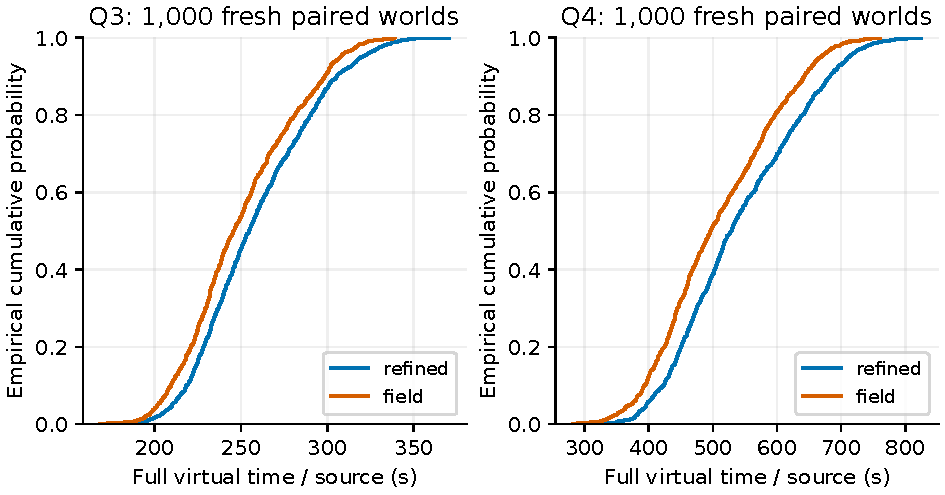
\includegraphics[width=\textwidth]{field_performance.pdf}
\caption{主组refined与field的单源耗时累积分布}
\label{fig:performance}
\end{figure}
图\ref{fig:performance}中曲线在同一累计比例下越靠左，表示相应分位点耗时越短。主组既有整体水平下降，也有尾部改善；二者与表\ref{tab:main}的均值和$p_{90}$一致。

\subsection{机制消融与成本组成}
Q3的主组采用逐步加入机制的配置链。仅更改路线时，平均耗时为254.07秒/源；加入预检测及负观测更新后为251.13秒/源；再加入安全接近后为250.17秒/源。相邻平均节省分别为4.92、2.94和0.96秒/源。这些增量对应当前配置链，反映机制之间的共同作用。

进一步把每个世界的总时间拆成五项，先分别除以本局成功清除数，再在世界间取平均，得到表\ref{tab:cost}。
\begin{table}[H]\centering\small
\setlength{\tabcolsep}{4.5pt}
\caption{主组单源费用分解，单位：秒/源}\label{tab:cost}
\CostResults
\end{table}
由表可见，移动仍是主要费用。Q3中field将每源移动成本由195.50降至188.36秒；Q4由383.47降至350.93秒。检测和换频费用也略有下降，说明路线改变会影响后续观测和任务顺序。

Q4失败清除尝试均值由1.782增至2.089次/局，但失败清除的单源费用增幅小于移动节省。因此不能只用失败次数判断策略优劣，仍需结合完整计时式。成功清除项在全清条件下固定为每源5秒。

\begin{figure}[htbp]\centering
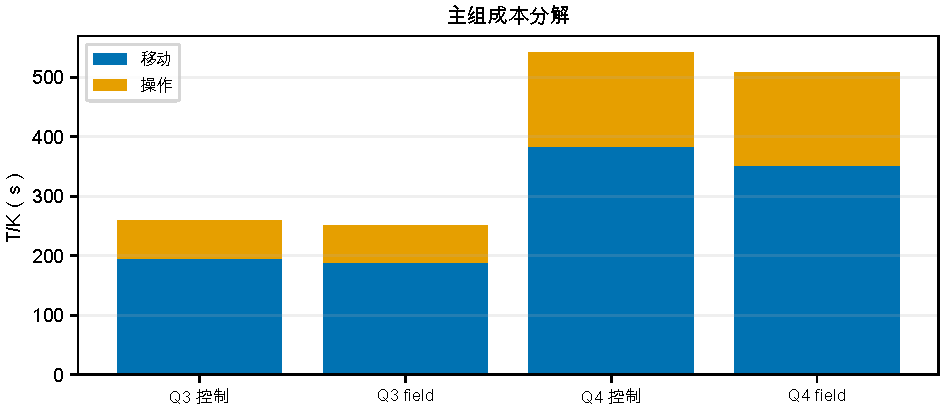
\includegraphics[width=0.97\textwidth]{competition_costs.pdf}
\caption{主组五项成本在两种策略中的组成}
\label{fig:cost}
\end{figure}

\subsection{官方演练结果}
旧refined策略的官方演练每题各10局，包含逐步请求、返回结果和测试结束后的源数量。结果见表\ref{tab:practice}。
\begin{table}[H]\centering\small
\caption{refined官方演练汇总，时间单位：秒/源}\label{tab:practice}
\PracticeResults
\end{table}
两题均完成全部源清除，移动分别占虚拟总时间的74.38\%和73.20\%。这一费用结构与本地试验中的移动主导现象一致，也是改进任务顺序的直接依据。

补充演练汇总中，Q3的field为11局、134个源，逐局平均263.550883秒/源；Q4为12局、166个源，逐局平均484.966300秒/源。这些案例与refined演练不同，尤其Q3平均源数由13.9降至约12.18，搜索固定费用分摊到每源后的影响随之变化。因此将两组演练作为运行表现观察，不把均值差当作同世界的算法节省。

前文以refined作为Q3基准、field作为Q4增强方案。以下正式测试的两题均采用field，按实际执行策略分别列示。

\section{正式测试结果}\label{sec:formal}
问题三和问题四各进行三次正式测试，均采用field策略。表中的$K$为成功清除源数，$T$为虚拟总时间；本机运行时间由控制程序测得，与模拟器界面计时分开列示。

\begin{table}[H]\centering\small
\setlength{\tabcolsep}{4pt}
\caption{问题三正式测试结果（field）}\label{tab:formal-q3}
\FormalThree
\end{table}
Q3三局共成功清除\FormalThreeK{}个源，虚拟总时间合计\FormalThreeT{}秒。逐局单源时间由215.647至270.163秒不等；三局等权平均为\FormalThreeMean{}秒/源，汇总指标为\FormalThreePooled{}秒/源。两种均值的差别来自各局成功清除数量不同。

\begin{table}[H]\centering\small
\setlength{\tabcolsep}{4pt}
\caption{问题四正式测试结果（field）}\label{tab:formal-q4}
\FormalFour
\end{table}
Q4三局共成功清除\FormalFourK{}个源，虚拟总时间合计\FormalFourT{}秒。逐局等权平均为\FormalFourMean{}秒/源，汇总指标为\FormalFourPooled{}秒/源。第三局成功清除数较少，单源时间较高，说明总时间和源数都影响$T/K$。

六局均满足各频道完成清除或无源判断的停止条件。正式测试未提供每局真实源数，故只报告成功清除数、虚拟时间和停止状态，不计算清除率；该结果与第\ref{sec:experiments}节的合成配对试验分开统计。

图\ref{fig:formal-compare}并列展示六局正式测试的单源时间，并标出各局成功清除数$K$。虚线分别表示两题的逐局等权均值，图中只比较本次案例的耗时分布，不将不同案例视为配对策略试验。
\begin{figure}[htbp]\centering
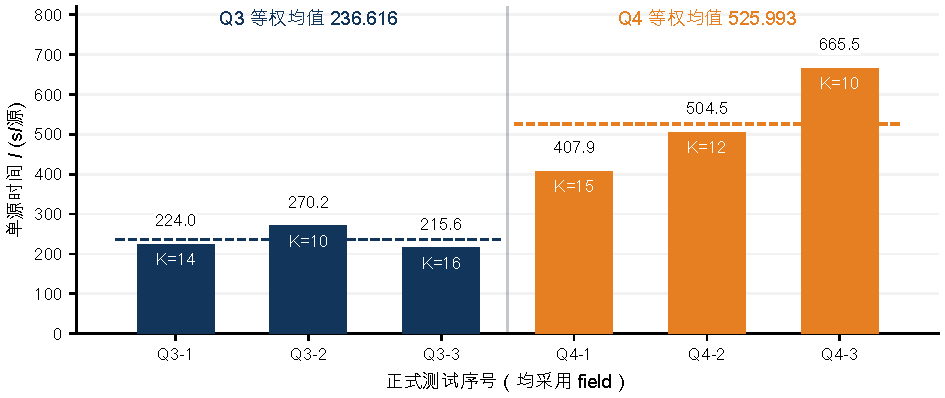
\includegraphics[width=\textwidth]{formal_compare.pdf}
\caption{六次正式测试的单源时间与成功清除数（均采用field）}
\label{fig:formal-compare}
\end{figure}

\section{模型检验与灵敏度分析}
\subsection{定位与停止条件的检验}
位置可行域的核心性质是始终包含真实源。对此，使用2000组、每组4次测向的计算检查角度跨零、边界位置、端点误差及两位小数舍入；最小包围圆另与1、2、3个支持点的枚举结果进行504组交叉比较。

Q3负观测更新检查了3000次真实源包含情形及边界、退化区域。安全接近在200组区域上重新计算候选点到全部顶点的距离。Q4双环通过三角形边界连接、面积、无交叉及坐标余量核对，与方向覆盖推导相对应。

停止条件检验中，未知频道在全部骨架扫描完成后判断无源，已发现频道在清除成功后完成；拒绝动作不计入位置和扫描记录。再按实际移动、检测、换频及清除次数重算时间，与各步返回的虚拟时刻一致。

\subsection{边界位置与不同误差场}
设置三类位置情形：全部源接收半径为1000米；16个源位于圆周，Q4其中15个朝外发射；16个源聚集在距圆心1650米附近的35米小圆盘中。每类分别使用三种误差场，每组50对世界。另对随机位置的两种替代误差各使用200对世界。

\begin{table}[H]\centering\small
\setlength{\tabcolsep}{3.5pt}
\caption{Q3边界与替代误差测试，时间单位：秒/源}\label{tab:stress-q3}
\StressThree
\end{table}
Q3全部组完成全清。最小接收半径组的平均节省较大，说明在接收余量较小时，观测与路线的配合仍有效。圆周和聚集组的节省较小：前者的固定扫描位置作用更突出，后者则减少了任务间远距离移动，留给路线改进的空间相应缩小。

\begin{table}[H]\centering\small
\setlength{\tabcolsep}{3.5pt}
\caption{Q4边界与替代误差测试，时间单位：秒/源}\label{tab:stress-q4}
\StressFour
\end{table}
Q4全部组也完成全清。圆周朝外发射组检验了外环点的作用，在三类误差下均保持有效搜索。聚集平滑误差组的节省区间跨越0，当前50对样本未证实该组均值改善；其余结果结合位置结构分别解释，不作为每个场景均更快的结论。

\subsection{横向偏移比例的影响}
局部测向式\eqref{eq:flank}中，包围半径前的比例决定候选点离中心的距离。比例过小，交会改善有限；比例过大，移动和失信号风险增加。对refined取比例0.12、0.22和0.40，在每题50个相同世界上比较，结果见表\ref{tab:sensitivity}。
\begin{table}[H]\centering\small
\caption{横向偏移比例的灵敏度试验（refined），时间单位：秒/源}\label{tab:sensitivity}
\SensitivityResults
\end{table}
三种比例下各组均完成全清。均值的变化小于2秒/源，尾部耗时和失败尝试数也有变化，但没有随比例增大而一致改善的趋势。因此采用0.22作为既定参数。这组试验与field主比较使用不同案例，结果分别统计。

\subsection{局部搜索与整体耗时的关系}
最近插入、2-opt和单点搬移均对当前有限任务排列进行改进。小规模静态路线可以穷举全部排列作为对照，而在线任务会随着示向结果、域收缩和清除终点发生变化。两者的区别在于：静态路线只计算固定任务坐标，完整任务还包含定位与操作费用。

因此，判断算法效果时，一方面检查候选排列保留全部任务，另一方面比较逐世界的$T/K$、检测次数、换频次数和失败清除次数。表\ref{tab:cost}中Q4失败尝试上升而总时间下降，正体现了局部指标与总体费用的差别。

\section{模型评价与结论}
\subsection{模型的优点}
\begin{enumerate}
\item \textbf{定位与清除衔接明确。}用交会区域表示测向误差，再用最小包围圆判断一次清除，避免将方向读数直接当作精确坐标。
\item \textbf{搜索过程具有覆盖依据。}七点环解决全向距离覆盖，25点双环同时处理源位置和发射方向，圆周朝外发射情形包含在构造内。
\item \textbf{任务顺序随观测调整。}扫描点和定位任务共同排序，清除后从新位置继续选择任务，减少固定往返带来的行程。
\item \textbf{完成条件可逐频道检查。}成功清除、已发现未清除和完成覆盖后的无源状态分别记录，源数量未知时仍有明确的停止方式。
\end{enumerate}

\subsection{模型的不足与适用范围}
固定骨架便于证明覆盖，但没有充分利用所有已知源位置调整后续检测点；Q3负观测取凸外包后会填回部分已排除区域，损失一些信息；路线采用有限局部改进，对完整自适应任务没有全局最优保证。

数值试验的源位置和误差场是人为设置的合成分布，官方案例中的运行表现还受源分布、源数和发射方向影响。当前模型适用于静止源、已知接收上下界和有界示向误差条件。推广到其他区域尺度时，应同时调整检测骨架并重新核对覆盖距离，而不能仅按比例缩放所有经验参数。

\subsection{结论}
本文以交会可行域、固定覆盖骨架和联合调度完成四问求解。问题一给出区域分类和顶点直径算法，并用三角形反例说明直径圆不能总是覆盖；问题二得到三圆交安全候选域，以离散交会计算选择第二检测点；问题三和问题四分别采用七点环与25点双环，结合有限测向和矩形光学覆盖完成清除。

主组合成配对试验中，field相对refined的平均单源时间分别降低\QThreeGain\%和\QFourGain\%，全部主组和列示边界组均全清。六次正式测试采用field，Q3、Q4三局等权平均分别为\FormalThreeMean{}和\FormalFourMean{}秒/源，均按频道完成条件结束。

\clearpage
\section*{AI 工具使用声明}
本参赛队在竞赛过程中使用了AI工具，主要用于语言润色、代码调试等辅助工作，详细使用情况见支撑材料。
\thispagestyle{plain}
\clearpage
\begin{thebibliography}{99}
\raggedright
\bibitem{problem} 全国大学生数学建模竞赛组委会. 2026年高教社杯全国大学生数学建模竞赛B题：无线电干扰源的快速自动定位与清除，以及附件1、附件2[Z]. 2026.
\bibitem{welzl} Welzl E. Smallest enclosing disks (balls and ellipsoids)[C]//Maurer H, ed. New Results and New Trends in Computer Science. Lecture Notes in Computer Science, 555. Berlin, Heidelberg: Springer, 1991: 359--370. DOI: \nolinkurl{10.1007/BFb0038202}.
\bibitem{jung} Jung H. Ueber die kleinste Kugel, die eine räumliche Figur einschliesst[J]. Journal für die reine und angewandte Mathematik, 1901, 123: 241--257. DOI: \nolinkurl{10.1515/crll.1901.123.241}.
\bibitem{sutherland} Sutherland I E, Hodgman G W. Reentrant polygon clipping[J]. Communications of the ACM, 1974, 17(1): 32--42. DOI: \nolinkurl{10.1145/360767.360802}.
\bibitem{qin} 秦明峰, 郝青儒, 范广伟. 运动单站无源定位性能分析[J]. 无线电工程, 2014, 44(4): 50--53.
\bibitem{li} 李亚军. 机载塔康无源定位方法研究[J]. 无线电工程, 2019, 49(3): 229--233.
\bibitem{rosenkrantz} Rosenkrantz D J, Stearns R E, Lewis P M II. An analysis of several heuristics for the traveling salesman problem[J]. SIAM Journal on Computing, 1977, 6(3): 563--581. DOI: \nolinkurl{10.1137/0206041}.
\bibitem{croes} Croes G A. A method for solving traveling-salesman problems[J]. Operations Research, 1958, 6(6): 791--812. DOI: \nolinkurl{10.1287/opre.6.6.791}.
\bibitem{galceran} Galceran E, Carreras M. A survey on coverage path planning for robotics[J]. Robotics and Autonomous Systems, 2013, 61(12): 1258--1276. DOI: \nolinkurl{10.1016/j.robot.2013.09.004}.
\bibitem{wasserman} Wasserman L. All of Statistics: A Concise Course in Statistical Inference[M]. New York: Springer, 2004. DOI: \nolinkurl{10.1007/978-0-387-21736-9}.
\end{thebibliography}
\clearpage
\appendix
\section{附录：程序与支撑材料}
\subsection{核心运行与验证代码}
\lstinputlisting[language=Python,caption={规划器与统一运行入口}]{b_solution/planner.py}
\lstinputlisting[language=Python,caption={本地环境与模拟器接口}]{b_solution/environment.py}
\lstinputlisting[language=Python,caption={几何计算与覆盖工具}]{b_solution/geometry.py}
\lstinputlisting[language=Python,caption={官方接口客户端}]{b_solution/client.py}
\lstinputlisting[language=Python,caption={问题三、四策略实现}]{b_solution/field_policy.py}
\lstinputlisting[language=Python,caption={路线组合与负观测几何}]{b_solution/route_portfolio.py}
\lstinputlisting[language=Python,caption={本地实验与官方日志分析入口}]{b_solution/field_confirmation.py}
\lstinputlisting[language=Python,caption={统一打包与复现验证}]{b_solution/package.py}
\lstinputlisting[language=Python,caption={关键几何和状态核验}]{b_solution/verify_field.py}
\lstinputlisting[language=Python,caption={竞赛版图表生成}]{b_solution/make_competition_assets.py}
\lstinputlisting[language=Python,caption={任务调度与候选策略}]{b_solution/joint_dispatch_candidate.py}
\lstinputlisting[language=Python,caption={Q3负观测几何}]{b_solution/negative_geometry.py}
\lstinputlisting[language=Python,caption={Q3Q4实验运行}]{b_solution/field_study.py}
\lstinputlisting[language=Python,caption={问题一交会计算}]{b_solution/intersection.py}
\lstinputlisting[language=Python,caption={问题二测点示例}]{b_solution/second_point.py}
\lstinputlisting[language=Python,caption={覆盖点生成}]{b_solution/coverage.py}
\lstinputlisting[language=Python,caption={Q1、Q2图片重绘}]{b_solution/redraw_q1q2.py}
\lstinputlisting[language=Python,caption={Q3、Q4图片重绘}]{b_solution/redraw_q34.py}
\lstinputlisting[language=Python,caption={结果图片重绘}]{b_solution/redraw_results.py}
\lstinputlisting[language=Python,caption={新增正文图表生成}]{b_solution/redraw_additional.py}

\end{document}
